\section{Examples}
\label{sec:example}
We present examples for two cases of the online intervention. In both cases, the observer monitors the attacker and the users' actions. The user computes a plan for a desirable goal state, $G_d$. Given the unexpected modification to the domain, executing this precompiled plan may likely cause the user to reach the undesirable state ($G_u$).

\begin{figure}[ht]
	\centering{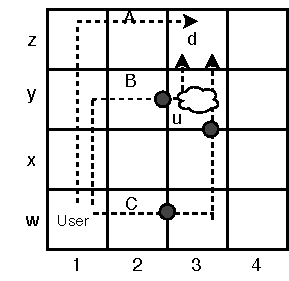
\includegraphics[width=\columnwidth]{single.pdf}}
	 \vspace{0.1mm}
	\caption{Reaching $G_u$ in a single agent environment}
	\label{fig:single}
\end{figure}


\textbf{Single agent}: We chose a grid navigation example to model intervention in a single agent environment. On a 4x4 grid shown in Figure \ref{fig:single}, an agent U is navigates by moving vertically and horizontally to reach a desired goal $G_d$. Initially, U is on cell (1,1). Let us assume U is optimal and will always choose the shortest path to reach $G_d$. On Figure \ref{fig:single} (1), paths A, B, and C are all optimal. However, cell (3,3) has a pit U can not see, which yeilds paths B and C unsafe as they lead to the undesirable state ($G_u$). The grid world also has an observer agent who has full observability of the domain, monitors U's actions and intervenes for the benefit of U. In Figure \ref{fig:single} (2), the observer has seen U take two steps to move to cell (1,3). From this position, there is no way for U to reach $G_d$ safely, while being optimal. Therefore, the observer must intervene when action of moving from (1,2) to (1,3) is observed. The prior two moves should not be flagged, as they are false alarms.


\textbf{Multi-agent}: 
We model an active adversary who attempts to make the user reach the undesirable state by leveraging the user's progress. We use the IPC block-words domain  \cite{gupta1992bw}. Figure \ref{fig:multi} shows the change in observer's beliefs as the user execute actions to spell different words. Figure \ref{fig:multi} (top) models a  scenario where 4 blocks: T, B, A, D are on the table. User's executes a plan to reach  $G_d=$TAD, while $G_u=$BAD. The user can not recognize block B (indicated by dotted lines), and therefore fails to circumvent $G_u$ on his own. The attacker will use block B to defeat the user and achieve $G_u$. Assuming both the user and the attacker are optimal, the observer must intervene when PICK-UP B is observed. Any subsequent action must also be flagged if it leads further toward $G_u$ (e.g., STACK B A). Figure \ref{fig:multi} (bottom) models a similar situation where $G_d=$CUP and $G_u=$CUT. The attacker stacks the hidden block T on P, which will lead to $G_u$ early in the observation sequence. In this case, the observer must intervene when STACK T P is observed. Any subsequent action leading  to $G_u$ must also be flagged.

\begin{figure}[tb]
	\centering{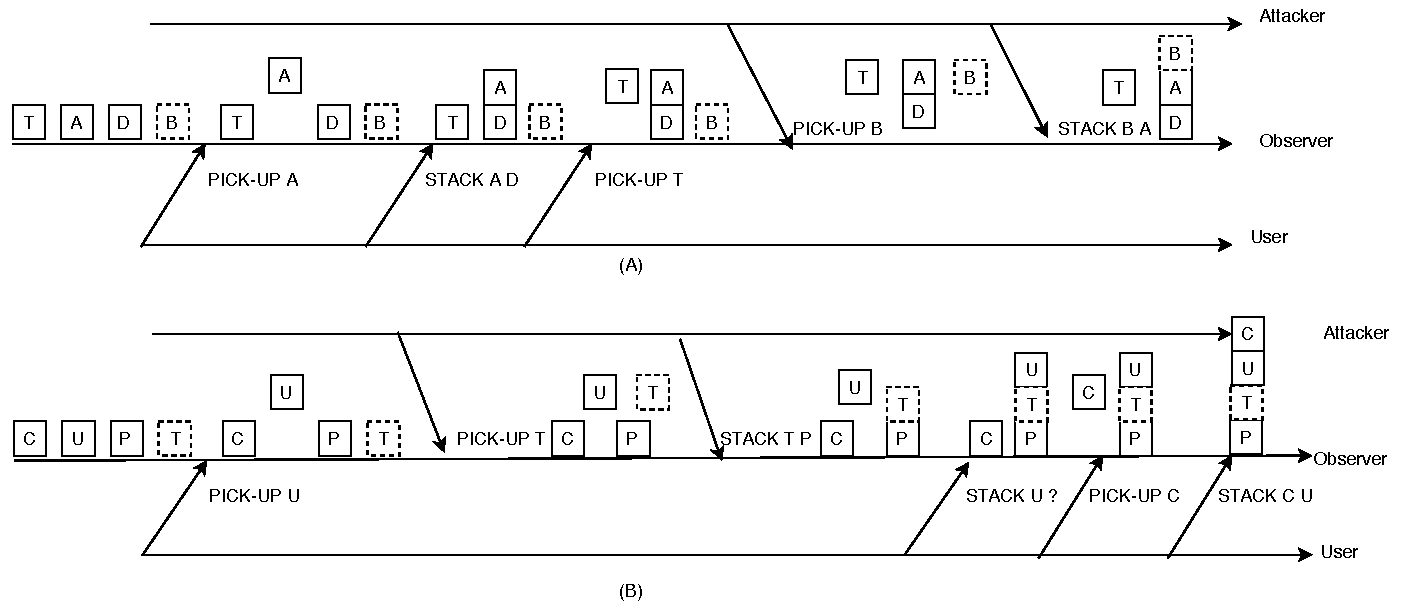
\includegraphics[width=\columnwidth]{multi.pdf}}
	\caption{Reaching $G_u$ with an active attacker}
	\label{fig:multi}
\end{figure}

%Figure \ref{fig:example} (right)  illustrates how the user's plans to reach $G_d$ could fail. In this case, given the assumption that the attacker does not backtrack to a previous state and only leverages progress made thus far, it can make four attempts to prevent the user from reaching $G_u$ by inserting the hidden block into the partially built stack. If the user achieves goal states 1 or 4 the user wins despite the attacker. If the observed actions indicate that the user is heading toward one of these two states, then an interrupt is unwarranted. State 3 is less ideal for the user but $G_u$ is not achieved. In state 2 the attacker has successfully reached $G_u$. Observations indicating state 2 warrant interruption.